\documentclass[letterpaper,11pt]{report}
\usepackage{xeCJK}
\usepackage{bm}
\usepackage{geometry}
\usepackage{amssymb}
\usepackage{amsmath}
\usepackage[cal=boondoxo, scr=dutchcal]{mathalfa}
\usepackage{multirow}
\usepackage[unicode, CJKbookmarks=true]{hyperref}

\numberwithin{equation}{section}

\geometry{a4paper,left=2cm,right=2cm,top=2cm,bottom=2cm}

\usepackage{setspace}
\setstretch{1.1}
\setlength{\parskip}{0.1\baselineskip}

\usepackage{graphicx}
\usepackage{caption}

\begin{document}

\title{CS229 Lecture Notes}
\author{Andrew Ng and Tengyu Ma}
\maketitle

% 监督学习
\part{监督学习}

% chapter 线性回归
\chapter{线性回归}

为了让我们的住房案例更有趣,让我们考虑一个稍微复杂些的数据集,我们额外知晓每套住房的卧室数量:

\begin{center}
  \begin{tabular}{c|c|c}
    居住面积(平方英尺) & \#卧室数量 & 价格(1000美元) \\
    \hline
    2104                 & 3          & 400              \\
    1600                 & 3          & 330              \\
    2400                 & 3          & 369              \\
    1416                 & 2          & 232              \\
    3000                 & 4          & 540              \\
    $\vdots$             & $\vdots$   & $\vdots$         \\
  \end{tabular}
\end{center}

其中,$x$为属于$\mathbb{R}^2$的二维向量。例如,$x_1^{(i)}$为训练集中第$i$套住房的居住面积,$x_2^{(i)}$为其卧室数量。(通常,当设计一个学习问题时,需要由你自己来决定选择哪些特征,因此,如果你在波特兰(Portland)收集住房数据,可能也会选择其他特征,比如,每套住房是否有壁炉及浴室的数量等。我们后续会讨论更多有关于特征选择的内容,但目前只考虑上面给出的特征。)

为了开展监督学习,我们必须决定如何在计算机中表示函数或假设$h$。作为初始选择,我们将$y$近似为一个关于$x$的线性函数:
$$
  h_\theta(x)=\theta_0+\theta_1 x_1 + \theta_2 x_2
$$
其中,$\theta_i$为参数(也称为权重),参数化从$\mathscr{X}$映射到$\mathcal{Y}$的线性函数空间。我们将$h_\theta(x)$简写为$h(x)$。为了简化我们的表示,我们引入$x_0=1$(截距项,Intercept Term),可以得到如下等式:
$$
h(x)=\sum^d_{i=0}\theta_i x_i = \theta^T x
$$
其中,我们可以将上述等式右侧的$\theta$与$x$视为向量,$d$为输入变量的数量(不计算$x_0$)。

% LMS 算法
\section{LMS算法}

我们需要找到一个$\theta$使$J(\theta)$最小化。让我们使用一种搜索算法,该算法以一个对$\theta$的初始猜测值开始,然后不断调整$\theta$使$J(\theta)$更小,直至收敛至某一个能够使$J(\theta)$最小化的$\theta$。特别地,让我们考虑梯度下降(Gradient Descent)算法,以某个初始值$\theta$开始,不断进行如下更新:
$$
  \theta_j:=\theta_j-\alpha\frac{\partial J(\theta)}{\partial \theta_j}
$$
(同时对所有$j=0,\ldots,d$使用此更新。)其中,$\alpha$被称为学习率,这是一个非常自然的算法,每次向$J$最陡峭的衰减方向前进一步。




% chapter 分类与逻辑回归
\chapter{分类与逻辑回归}

% 多分类问题
\section{多分类问题}

考虑这样一个分类问题,响应值$y$满足$y\in\{1,2,\ldots,k\}$。举个例子,我们可能想要将邮件划分为三种类型,比如垃圾邮件、个人邮件及工作邮件,而不是只划分为垃圾邮件与非垃圾邮件(这是一个二分类问题)。标签或响应值仍然是离散的,但可以取两个以上的值。因此我们将使用多项式分布对这种问题进行建模。

在这种情况下,$p(y | x;\theta)$是基于$k$个离散值的分布,这是一个多项式分布。对于包含$k$个值的多项式分布,$\phi_1,\ldots,\phi_k$表示每一种可能的概率,必须满足$\sum^k_{i=1}\phi_i=1$。我们将设计一个参数化模型,在给定输入$x$的前提下,输出满足这个约束的$\phi_1,\ldots,\phi_k$。

我们引入$k$组参数$\theta_1,\ldots,\theta_k$,每一组参数都是空间$\mathbb{R}^d$中的一个向量。根据直觉,我们应该可以使用$\theta_1^Tx,\ldots,\theta_k^Tx$来表示$\phi_1,\ldots,\phi_k$,即概率$P(y=1 | x;\theta),\ldots,P(y=k | x;\theta)$。然而,采用这种直接的办法有两个问题,首先,$\theta_j^Tx$不一定在$[0,1]$内,其次,$\sum^k_{j=1}\theta_j^Tx$不一定为$1$。因此,我们将使用softmax函数将向量$(\theta_1^T x,\ldots,\theta_k^T x)$转化为每个元素都是非负的并且和为$1$的概率向量。

定义softmax函数$\rm{softmax}:\mathbb{R}^k \rightarrow \mathbb{R}^k$为

\begin{equation}
  \rm{softmax}(t_1,\ldots,t_k)=
  \begin{bmatrix}
    \frac{{\rm{exp}} (t_1)}{\sum^k_{j=1}{\rm{exp}} (t_j)} \\
    \vdots                                                \\
    \frac{{\rm{exp}} (t_k)}{\sum^k_{j=1}{\rm{exp}} (t_j)} \\
  \end{bmatrix}
\end{equation}

softmax函数的输入,向量$t$一般被称为logits,在定义中,softmax函数的输出必为每个元素都是非负的并且和为$1$的概率向量。

令$(t_1,\ldots,t_k)=(\theta_1^Tx,\ldots,\theta_k^Tx)$,将$(t_1,\ldots,t_k)$作为softmax函数的输入,将softmax函数的输出作为概率$P(y=1 | x;\theta),\ldots,P(y=k | x;\theta)$,得到如下概率模型:
\begin{equation}
  \begin{bmatrix}
    P(y=1 | x;\theta) \\
    \vdots            \\
    P(y=k | x;\theta) \\
  \end{bmatrix}
  =
  \rm{softmax}(t_1,\ldots,t_k)
  =
  \begin{bmatrix}
    \frac{{\rm{exp}} (\theta_1^T x)}{\sum^k_{j=1}{\rm{exp}} (\theta_j^T x)} \\
    \vdots                                                                  \\
    \frac{{\rm{exp}} (\theta_k^T x)}{\sum^k_{j=1}{\rm{exp}} (\theta_j^T x)} \\
  \end{bmatrix}
\end{equation}
为了表示方便,我们令$\phi_i=\frac{{\rm{exp}} (\theta_i^T x)}{\sum^k_{j=1}{\rm{exp}} (\theta_j^T x)}$,上面等式可以简写为:
\begin{equation}
  P(y=i|x;\theta) = \phi_i= \frac{{\rm{exp}} (t_i)}{\sum^k_{j=1}{\rm{exp}} (t_j)} = \frac{{\rm{exp}} (\theta_i^T x)}{\sum^k_{j=1}{\rm{exp}} (\theta_j^T x)}
\end{equation}
接下来,我们计算一个样例$(x,y)$的负对数-似然(log-likehood)。
\begin{equation}
  -\log P(y|x,\theta)=-\log \left( \frac{{\rm{exp}} (t_y)}{\sum^k_{j=1}{\rm{exp}} (t_j)} \right) = -\log \left( \frac{{\rm{exp}} (\theta_y^T x)}{\sum^k_{j=1}{\rm{exp}} (\theta_j^T x)} \right)
\end{equation}
因此,训练数据的负对数-似然,即损失函数可以写为:
\begin{equation} \label{multi-class-loss}
  \mathcal{l}(\theta) = \sum^n_{i=1} - \log \left( \frac{{\rm{exp}} (\theta_{y^{(i)}}^T x^{(i)})}{\sum^k_{j=1}{\rm{exp}} (\theta_j^T x^{(i)})} \right)
\end{equation}
通过模块化上面的等式,可以很方便地定义交叉熵损失(Cross-entropy Loss)$\mathcal{l}_{ce}:\mathbb{R}^k \times \{1,\ldots,k\} \rightarrow \mathbb{R}_{\leq 0}$为:\footnote{这里的命名有些许歧义。一些人将交叉熵损失定义为将概率向量(在我们的定义中为$\phi$)与标签$y$映射为一个实数的函数,称我们的交叉熵损失为softmax-交叉熵损失。我们选择这种命名习惯是因为它与大多数现代深度学习库是一致的,比如PyTorch与Jax。}
\begin{equation}
  \mathcal{l}_{ce}((t_1,\ldots,t_k),y)=-\log \left( \frac{{\rm exp}(t_y)}{\sum^k_{j=1}{\rm{exp}} (t_j)} \right)
\end{equation}
通过上述等式,我们可以将等式\eqref{multi-class-loss}简写为:
\begin{equation}
  \mathcal{l}(\theta) = \sum^n_{i=1} \mathcal{l}_{ce}((\theta_1^T x^{(i)},\ldots,\theta_k^T x^{(i)}),y^{(i)})
\end{equation}
并且交叉熵损失也具有一个简单的梯度表示。令$t=(t_1,\ldots,t_k)$,且$\phi_i=\frac{{\rm exp}(t_i)}{\sum^k_{j=1}{\rm exp}(t_j)}$,通过基本微积分,我们可以推导出:
\begin{equation}
  \frac{ \partial \mathcal{l}_{ce}(t,y)}{\partial t_i}=\phi_i - 1 \{ y=i \}
\end{equation}
% TODO: add ref
其中,$1\{\cdot\}$为指示函数(Indicator Function),即如果$y=i$,$1\{y=i\}=1$,如果$y \ne i$,$1\{y=i\}=0$。另外,基于矢量表示法我们有如下表示法,该表示在第7节非常有用:
\begin{equation}
  \frac{ \partial \mathcal{l}_{ce}(t,y)}{\partial t_i}=\phi_i - e_s
\end{equation}
其中,$e_s \in \mathbb{R}^k$为第$s$个自然基向量(Natural Basis Vector,向量的第$i$个元素为$1$,其他元素为$0$),使用链式法则,我们可以得到:
\begin{equation}
  \frac{\partial \mathcal{l}_{ce}((\theta_1^T x,\ldots,\theta_k^T x),y)}{\partial \theta_i}=\frac{ \partial \mathcal{l}_{ce}(t,y)}{\partial t_i} \cdot \frac{t_i}{\theta_i} = (\phi_i - 1 \{ y=i \}) \cdot x
\end{equation}
因此,损失函数相对于参数$\theta_i$的的梯度为:
\begin{equation}
  \frac{ \partial \mathcal{l}(\theta)}{\partial \theta_i} = \sum^n_{j=1} (\phi_i^{(j)} - 1 \{ y^{(j)}=i \}) \cdot x^{(j)}
\end{equation}
其中,$\phi_i^{(j)}=\frac{{\rm{exp}} (\theta_{i}^T x^{(j)})}{\sum^k_{s=1}{\rm{exp}} (\theta_s^T x^{(j)})}$为模型将样例$x^{(j)}$预测为$i$的概率。根据上面的梯度公式,可以实现(随机)梯度下降以最小化损失函数$\mathcal{l}(\theta)$。


% Another algorithm for maximizing \mathcal{l}(\theta)
\section{最大化$\mathcal{l}(\theta)$的另一种算法}

回到逻辑回归问题,$g(z)$为sigmoid函数,让我们讨论另一种用于最大化$\mathcal{l}(\theta)$的算法。

让我们开始吧,考虑使用牛顿法寻找函数的零点。假设我们有一个函数$f:\mathbb{R}\rightarrow\mathbb{R}$,期望找到一个值$\theta$满足$f(\theta)=0$,其中$\theta \in \mathbb{R}$为实数。牛顿法进行如下操作:
$$
  \theta := \theta - \frac{f(\theta)}{f^\prime(\theta)}
$$
这个方法可以视为,在当前猜测值$\theta$处,通过一个正切于$f$的线性函数近似$f$,以求解该线性函数的零值,然后将下一个$\theta$设置为线性函数的零值。

\begin{figure}
  \begin{center}
    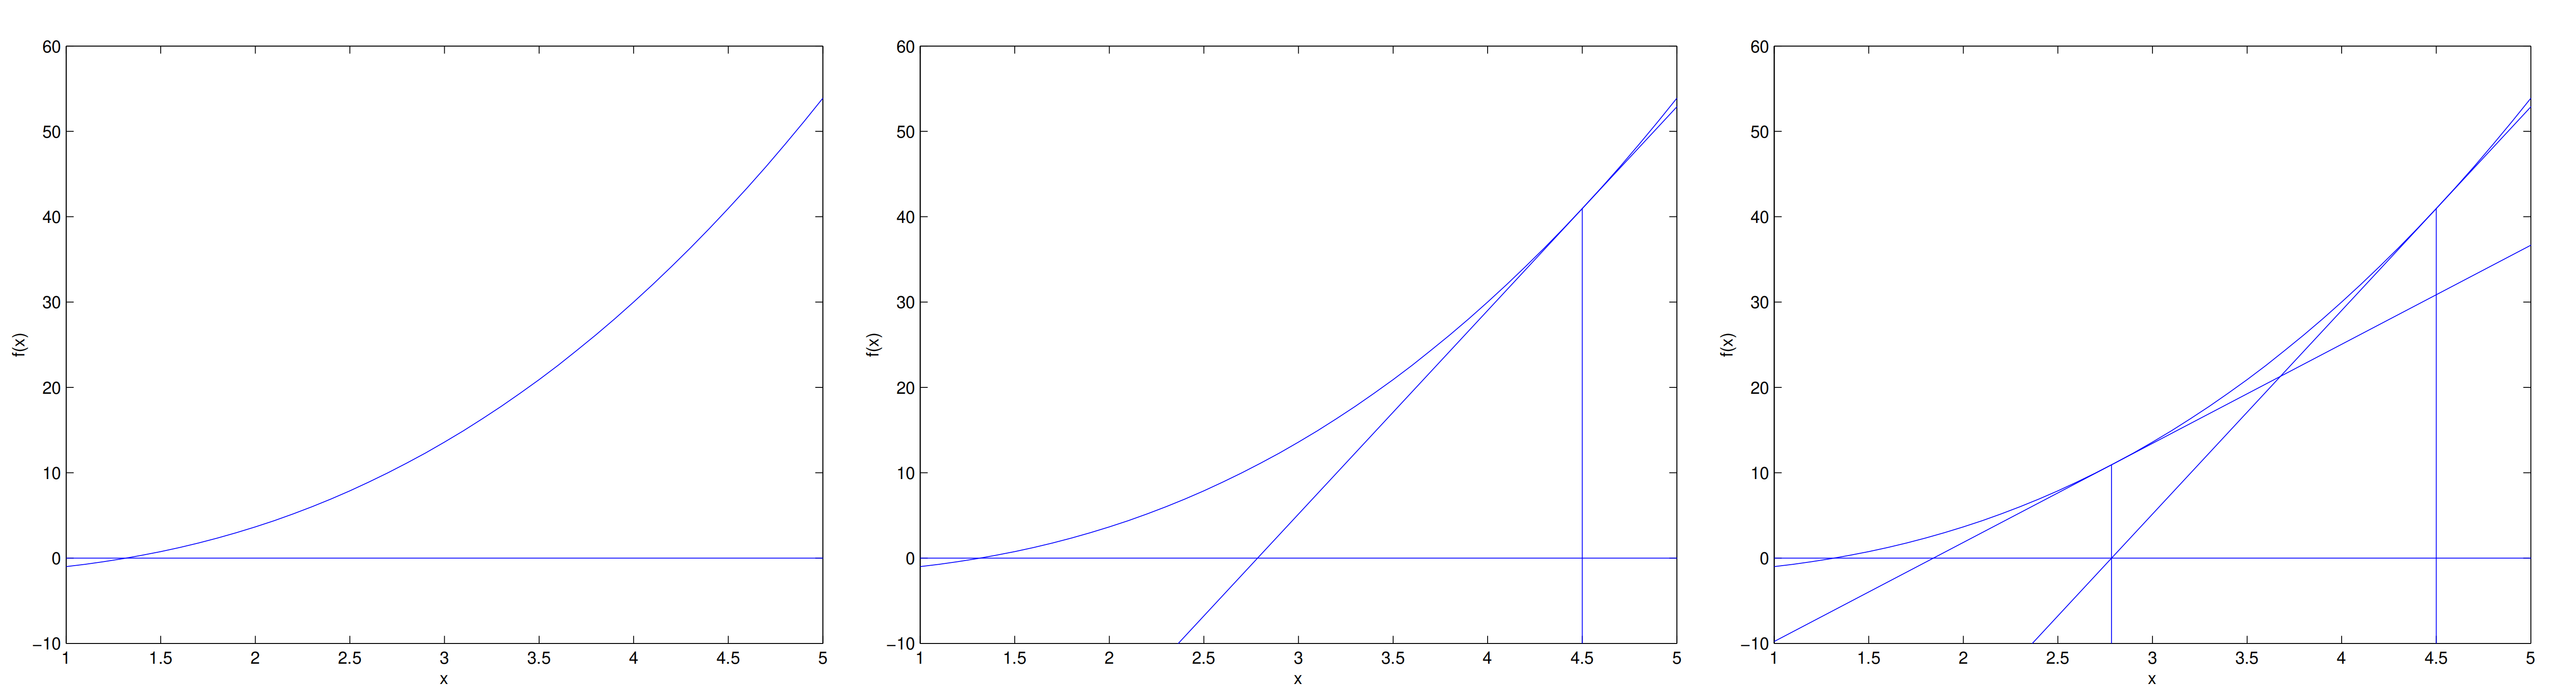
\includegraphics[width=0.9\textwidth]{imgs/2.4_newton.jpg}
  \end{center}
\end{figure}

这里有一张展示牛顿法具体步骤的图片:

在最左边的图片中,可以看到函数$f$与直线$y=0$绘制在一起,我们尝试寻找满足$f(\theta)=0$的$\theta$,能够满足这个目标的$\theta$约为$1.3$。假设我们设置$\theta$为$4.5$初始化此算法。




\end{document}
